\documentclass{article}

% A poster/flyer for the SemEval-2017 shared task on puns, for
% distribution at the 28th Conference of the International Society for
% Humor Studies (ISHS 2016)
%
% Typeset by Tristan Miller <http://www.nothingisreal.com/>
% June 2016
% 
% This source code is released under the Creative Commons
% Attribution 4.0 International (CC BY 4.0) licence.

\usepackage[hidelinks]{hyperref}
\usepackage[a4paper,hmargin=15mm,vmargin=30mm]{geometry}
%\usepackage[letterpaper,hmargin=15mm,vmargin=30mm]{geometry}
\usepackage[svgnames]{xcolor}
\usepackage{fontspec}
\usepackage{xunicode}
\usepackage{microtype}
\usepackage{tabularx}
\let\ifpdf=\ifxetex\usepackage{tikzrput}
\usepackage[object=vectorian]{pgfornament}
\usepackage{graphicx}
\defaultfontfeatures{Ligatures=TeX}
\setmainfont[RawFeature={+ss05,+dlig,+hlig,+calt,+liga},ItalicFeatures={RawFeature={+cv04,+clig,+swsh,+calt,+liga,+hlig,+ss05},CharacterVariant=5:0}]{EB Garamond}
\newcommand{\h}[1]{\textcolor{FireBrick}{#1}}
\pagestyle{empty}
\usepackage{parskip}
\begin{document}
\centering

\Huge \textsc{A \h{C}all for \h{P}articipation}

\vfill

\Large \emph{is hereby issued for a}

\vfill

\Huge \raisebox{0.4\height}{\pgfornament[scale=.35]{50}} \hspace{1ex} \scalebox{1.5}{\textsc{\h{S}hared \h{T}ask}} \hspace{1ex} \raisebox{0.4\height}{\pgfornament[scale=.35]{51}}

\vfill

\Large \emph{on the}

\vfill

\Huge \scalebox{1.25}{\textsc{\h{C}omputational \h{D}etection} \emph{\&}}\\
\scalebox{1.25}{\textsc{\h{I}nterpretation} \emph{of}}

\vspace{-10mm}
\begin{tabularx}{\linewidth}{cXc}%
\raisebox{-0.1\height}{%
\reflectbox{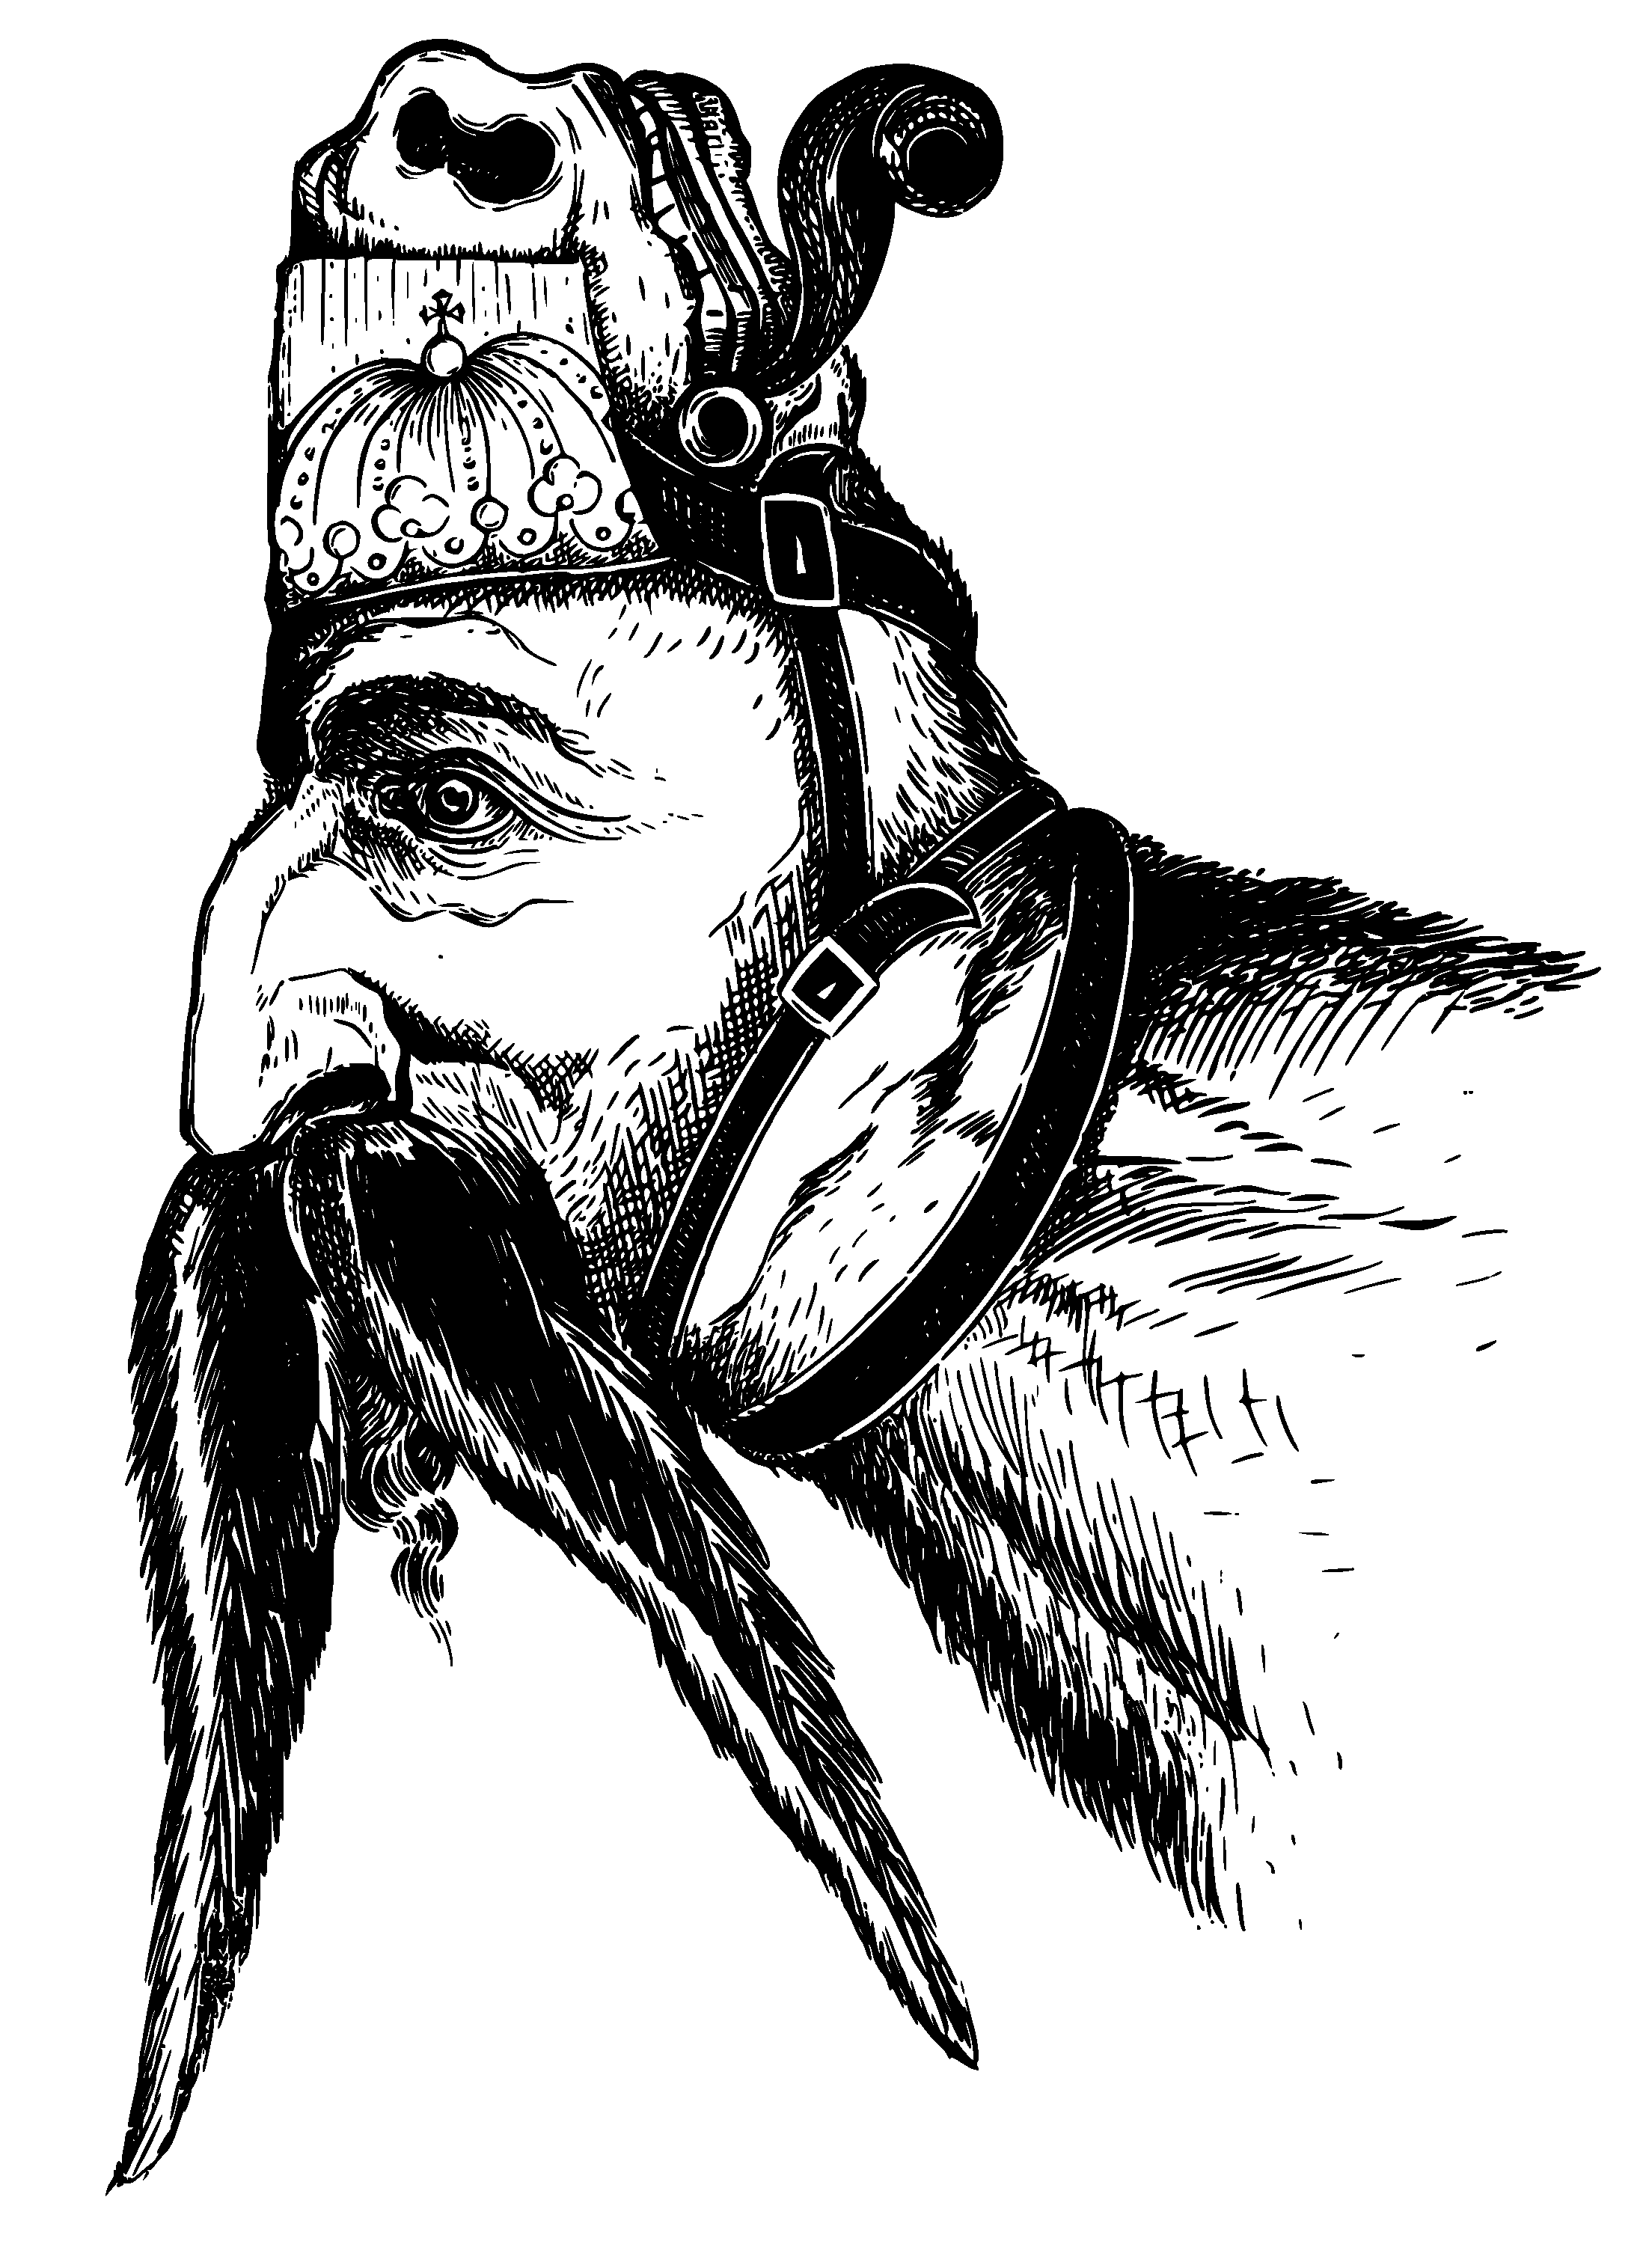
\includegraphics[width=30mm]{Badinguet}}%
}%
&%
\scalebox{5.5}{\Huge \h{PUNS}}&%
\raisebox{-0.05\height}{%
\reflectbox{\rotatebox[origin=c]{180}{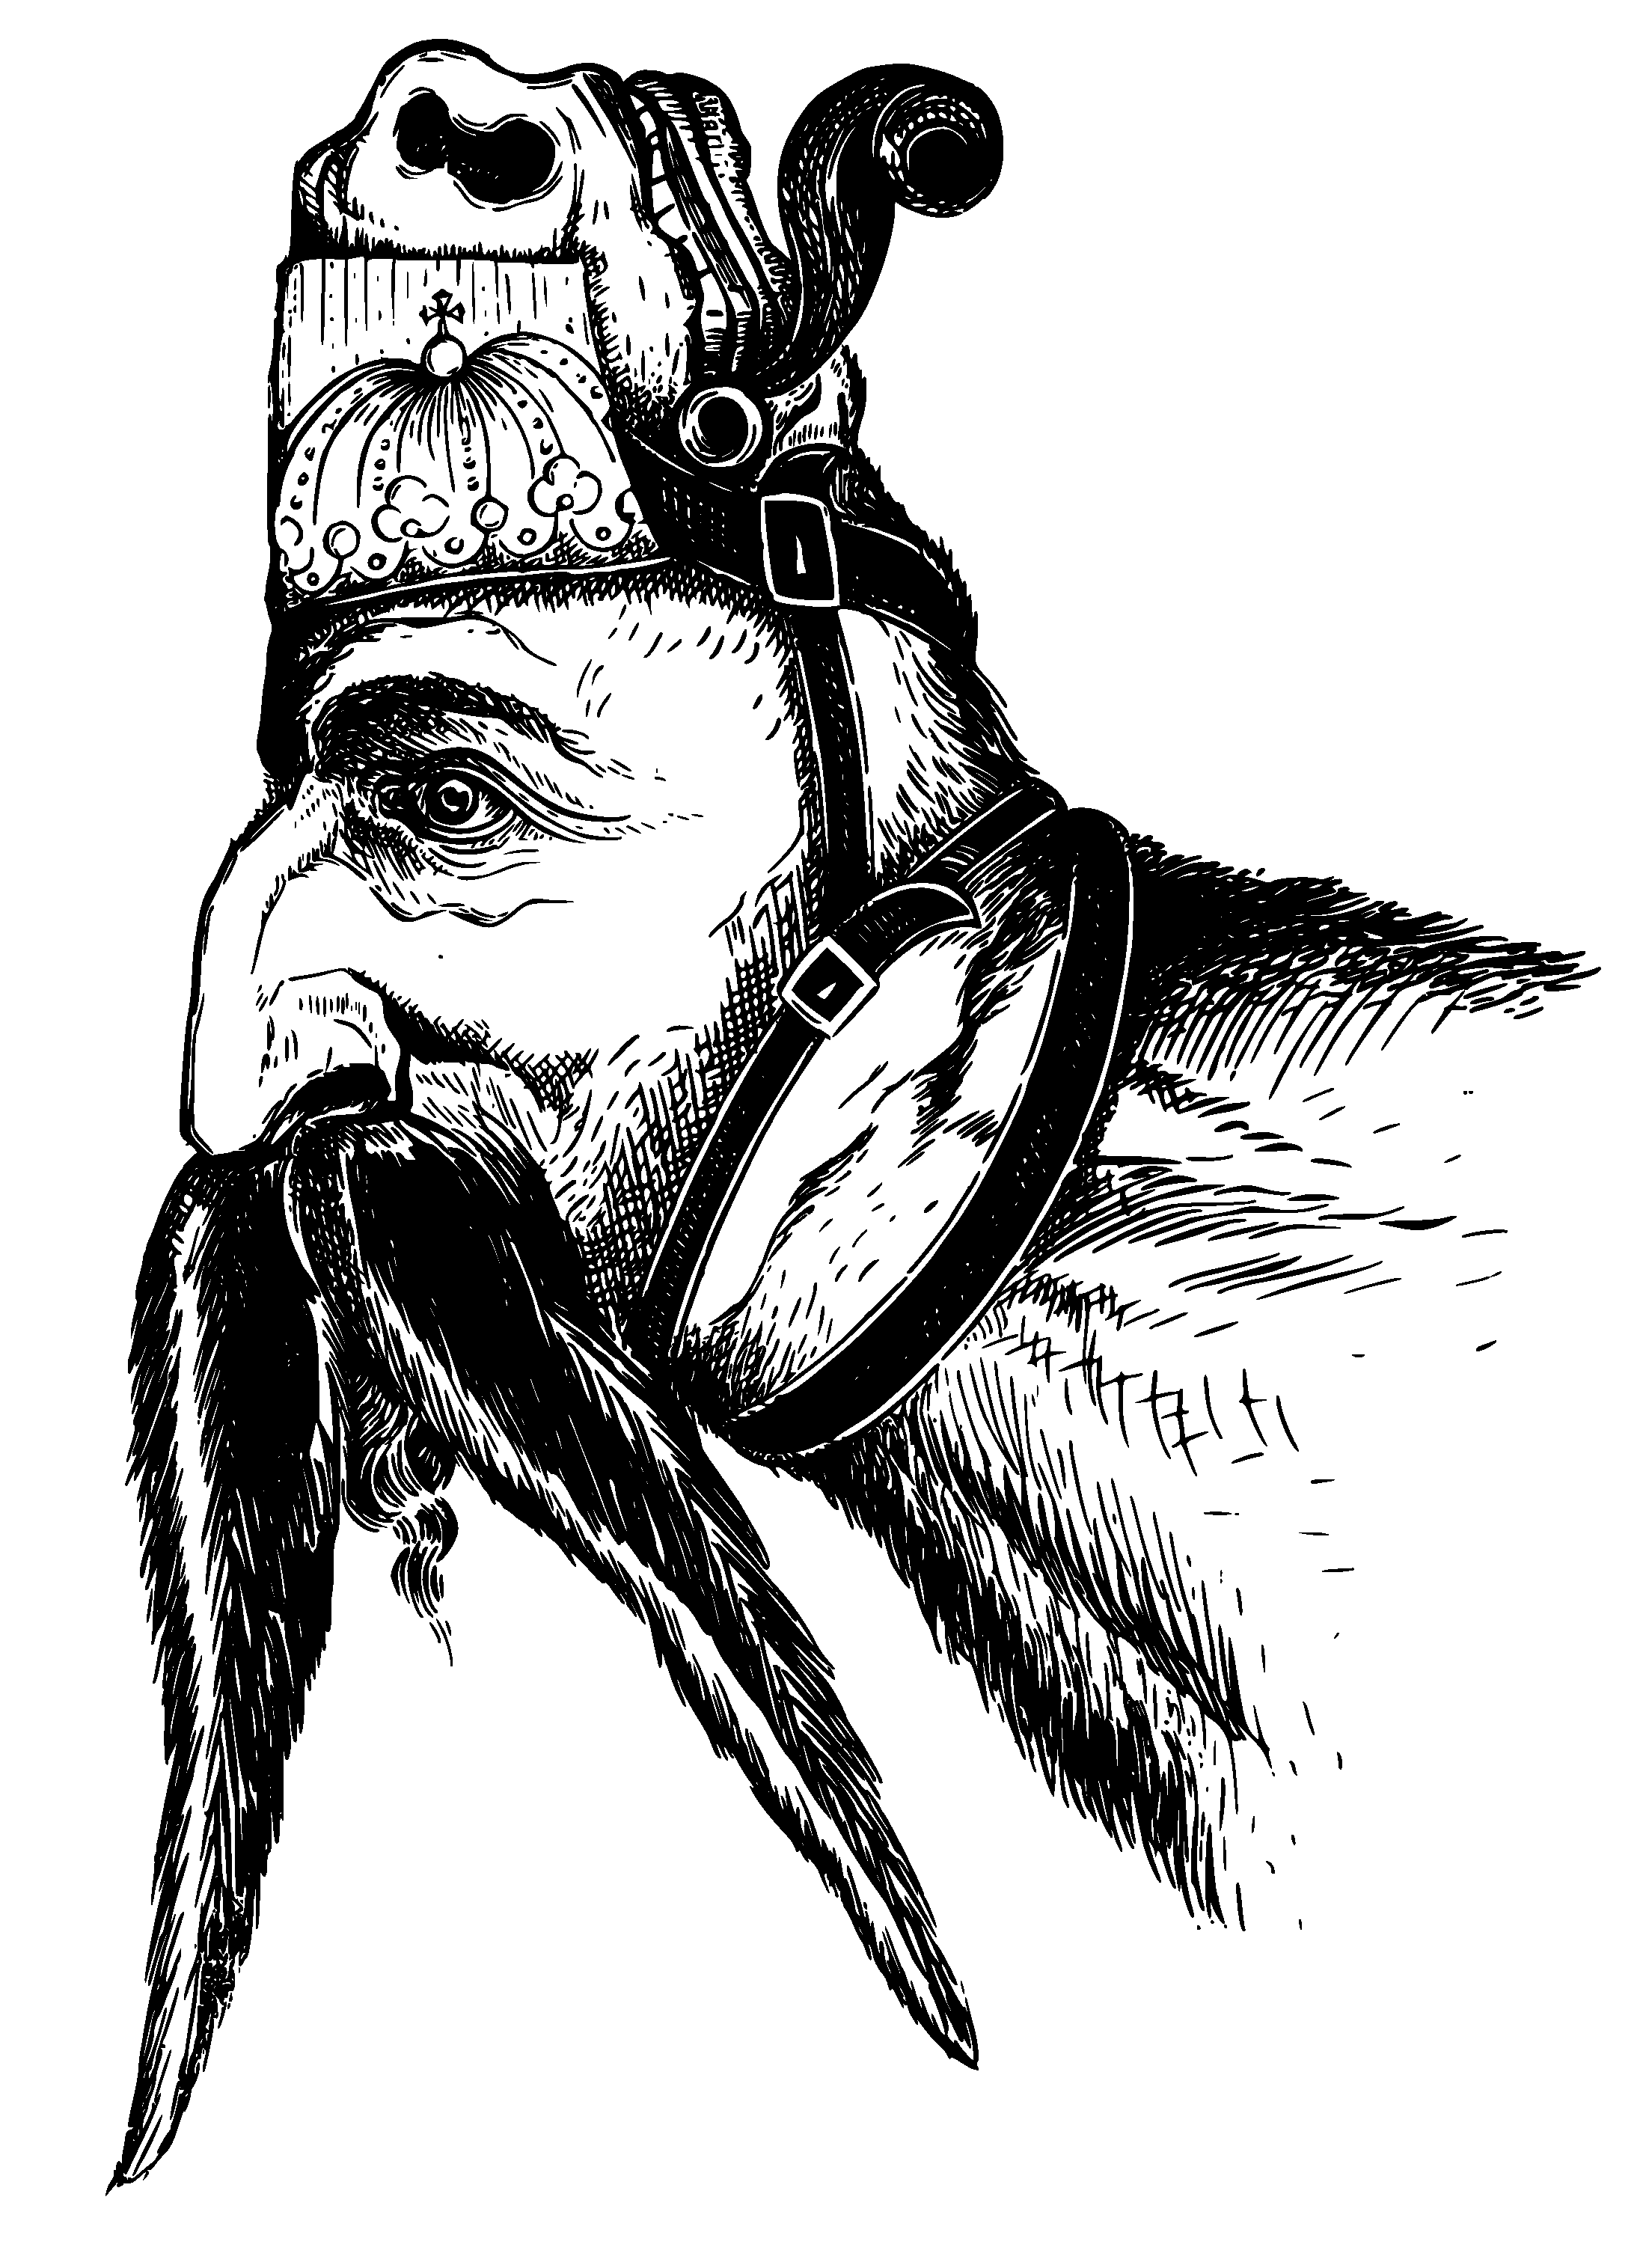
\includegraphics[width=30mm]{Badinguet}}}%
}%
%\\
\end{tabularx}

\vfill

\Large \emph{to be held at}

\vfill

\Huge \scalebox{3}{\textsc{\h{S}em\h{E}val-2017.}}

\vfill

\parbox{121mm}{\Large \textsc{SemEval} is an ongoing series of
  evaluations of computational semantic analysis sytems, organized
  under the ægis of \h{\textsc{Siglex}}, the \h{Special Interest Group
    on the Lexicon} of the \h{Association for Computational
    Linguistics}.  \textsc{SemEval-2017} will be co-located with a
  major \textsc{nlp} conference (\textsc{tba}) in the summer of
  2017.\linebreak}

\vfill

\Huge \textsc{For further information, visit:} \\
\Huge \raisebox{0.4\height}{\pgfornament[scale=.35]{15}} \hspace{1ex} \scalebox{1}{\h{\href{https://logological.org/puns}{https://{\kern3pt}logological.org/{\kern2pt}puns}}} \hspace{1ex} \raisebox{0.4\height}{\pgfornament[scale=.35]{16}}
\end{document}

%%% Local Variables:
%%% mode: latex
%%% TeX-PDF-mode: t
%%% TeX-engine: xetex
%%% TeX-master: t
%%% End:
